\subsection{Megtenni szándékozott lépések}

\begin{frame}{Megtenni szándékozott lépések}
	
	\begin{itemize}
		
		\item Wikipedia alapú WSD-rendszer felépítése
		\begin{enumerate}
			\item Egyik legnagyobb létező adathalmaz
			\item Több nyelven elérhető
			\item A cikkek címei conceptként való felhasználása
		\end{enumerate}
		
		\item WSD-rendszer integrálása a létező SMT-rendszerekbe
		\begin{enumerate}
			\item Statisztikai modellek nem veszik figyelembe a  többértelmű szavakat
			\item A fordítás pontossága nagyban növelhető lenne ezen problémák megoldásával
		\end{enumerate}
		
	\end{itemize}

\end{frame}

\newcounter{enumcounter}
\newcommand{\savecounter}{\setcounter{enumcounter}{\theenumi}}
\newcommand{\restorecounter}{\setcounter{enumi}{\theenumcounter}}

\begin{frame}{Megtenni szándékozott lépések}
\framesubtitle{Wikipedia alapú WSD-rendszer}

		\begin{enumerate}
			\item Invertált index felépítése minden nyelv számára	
			\begin{itemize}
				\item Minden szóhoz hozzárendelünk concepteket és a hozzájuk tartozó súlyt
				\item A conceptek az angol Wikipedia címek
				\item Súlyozáshoz használhatjuk például a tf-idf súlyozást
			\end{itemize}			
			
		\begin{figure}[t]
			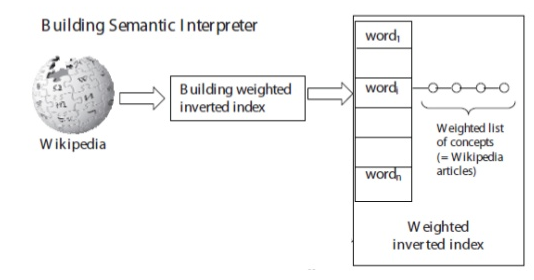
\includegraphics[scale=0.4]{images/invindex}
 		\end{figure}			
			
			\savecounter	
		\end{enumerate}

\end{frame}

\begin{frame}{Megtenni szándékozott lépések}
\framesubtitle{Wikipedia alapú WSD-rendszer}

	\begin{enumerate}
		\restorecounter
		
		\item Súlyozott concept- vektor hozzárendelése a fordítandó és SMT által fordított szöveghez
		\begin{itemize}
			\item Szöveg szavak vektoraként való ábrázolása 
			\item Conceptek megfelelő súllyal történő hozzárendelése minden szóhoz
			\item Ősszesített súlyozott concept- lista felépítése a szöveghez
		\end{itemize}
		
		\begin{figure}[t]
			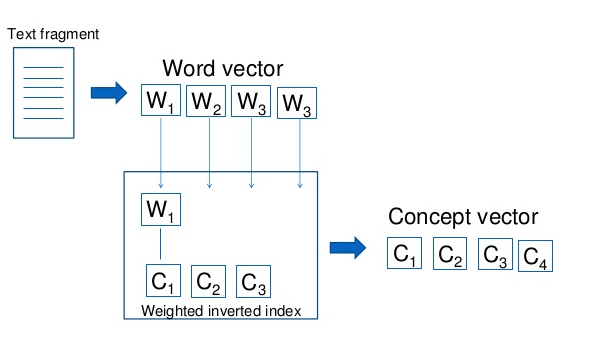
\includegraphics[scale=0.4]{images/textfragment}
 		\end{figure}			
 		
	\savecounter
 	
	\end{enumerate}
	
\end{frame}

\begin{frame}{Megtenni szándékozott lépések}
\framesubtitle{Wikipedia alapú WSD-rendszer}

	\begin{enumerate}
		\restorecounter	
	
		\item A szemantikai hasonlóság meghatározza a fordítandó és célszöveg között
		\begin{itemize}
			\item A fordítandó- és célszöveghez felépítjük a concept vektorokat
			\item A hasonlóság vizsgálatát a vektorok összehasonlítása jelenti
			\item A hasonlósági metrika lehet például a gyakran használt cos-távolság
		\end{itemize}
	
		\begin{figure}[t]
			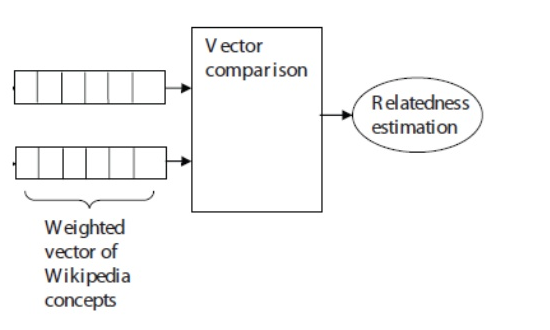
\includegraphics[scale=0.4]{images/similarity}
 		\end{figure}	
	
		\savecounter
	\end{enumerate}

\end{frame}

\begin{frame}{Megtenni szándékozott lépések}
\framesubtitle{WSD-súlyok integrálása}	
	
	\begin{enumerate}
		\restorecounter
						
		\item Legjobb N találat újrarangsorolása
		\begin{itemize}
			\item SMT-rendszer alapján meghatározni a legjobb N fordítást
			\item WSD-rendszer alapján súly hozzárendelése a találatokhoz
			\item A találatok újrarangsorolása az SMT és WSD együttes eredményei alapján
		\end{itemize}
	\end{enumerate}
	
\end{frame}